%\section{Problem 3.13}
\mysection{3.13}{Problem 3.13}

\numberwithin{equation}{subsection}

A Gaussian product channel $Y_j = g_j \cdot X_j + Z_j$ $j\in \{1,2\}$ with $g_1 < g_2$ and average power constraint $P$ is given. We want to know above what power $P^*$ we start to use both the channels and what are the features of the \textit{energy-per-bit-rate function} $E_b(R)$.

\subsection{Optimal power allocation}


We notiche that to achieve the maximum capacity from the channel we have to solve the following optimization problem.

\begin{equation}
\begin{gathered}
	\max_{P_j} \sum_{j=1}^2 \frac{1}{2} \cdot \log(1+g_j^2 \cdot P_j) \quad subject \quad to\\
	-P_j \neq 0 \quad j\in \{1,2\} \\
	\sum_{j=1}^2 P_j - P = 0
\end{gathered}
\label{optproblem}
\end{equation}

In order to solve \eqref{optproblem} we build the following equation.

\begin{equation}
	\nabla_{P_j}\Big\{-\sum_{j=1}^2 \frac{1}{2} \cdot \log(1+g_j^2 \cdot P_j) + \sum_{j=1}^2 \lambda_j \cdot (-P_j) + \nu \cdot \Big(\sum_{j=1}^2 P_j - P\Big)  \Big\} = 0
	\label{f0}
\end{equation}

Solving \eqref{f0} we obtain what follows.

\begin{equation}
	\begin{gathered}
		\frac{1}{2} \cdot \frac{1}{P_j+\frac{1}{g_j^2}}+\lambda_j-\nu=0 \\
		\Rightarrow \frac{1}{2} \cdot \frac{1}{P_j+\frac{1}{g_j^2}} \leq \nu = \frac{1}{2\mu}
	\end{gathered}
\end{equation}

\begin{equation}
	\begin{gathered}
		\sum_{j=1}^2 \max\Big\{\mu - \frac{1}{g_j^2},0\Big\} = P \\
		\Rightarrow \mu = \frac{P}{2}+\frac{1}{2g_1^2} + \frac{1}{2g_2^2}
	\end{gathered}
\end{equation}

\begin{equation}
	\begin{gathered}
	 P_j = \max\Big\{\mu - \frac{1}{g_j^2},0\Big\} \\
	 \Rightarrow P_1= \max\Big\{\frac{P}{2} + \frac{1}{2g_2^2} - \frac{1}{2g_1^2},0\Big\} = \begin{cases}
	  \frac{P}{2} + \frac{1}{2g_2^2} - \frac{1}{2g_1^2} \quad P \geq \frac{1}{g_1^2} - \frac{1}{g_2^2} \\
		0 \quad P < \frac{1}{g_1^2} - \frac{1}{g_2^2}
	 \end{cases} \\
	 \Rightarrow P_2= \max\Big\{\frac{P}{2} + \frac{1}{2g_1^2} - \frac{1}{2g_2^2},0\Big\} = \frac{P}{2} + \frac{1}{2g_1^2} - \frac{1}{2g_2^2} \quad \forall \quad P \geq 0
	\end{gathered}
\end{equation}

We conclude that the second channel is opened for every amount of allocated power $P$ while the first channel is opened only if and only if \eqref{Pcondition} is verified.

\begin{equation}
	P \geq \frac{1}{g_1^2} - \frac{1}{g_2^2}
	\label{Pcondition}
\end{equation}

\subsection{Energy-per-bit-rate function computation}

Now we want to compute the \textit{energy-per-bit-rate function} $E_b(R)$ in the scenario previously described. We know that $P = R \cdot E$ where $R$ is the \textit{bit-rate} of the channel and $E$ is the used energy for every bit. In addition we know that the \textit{bit-rate} is bounded by channel capacity as shown in \eqref{1case} and \eqref{2case}.

\begin{equation}
		R \leq \frac{1}{2} \cdot \log\big( 1 + g_2^2P \big) \Leftrightarrow P < \frac{1}{g_1^2} - \frac{1}{g_2^2}
		\label{1case}
\end{equation}


\begin{equation}
		R \leq \frac{1}{2} \cdot \sum_{j=1}^2 \log\Big(\frac{g_j^2}{2} \cdot \Big(P+\frac{1}{g_1^2} + \frac{1}{g_2^2}\Big)\Big)= \frac{1}{2} \cdot \log\Big(\frac{g_1^2 g_2^2}{4} \cdot \Big(P+\frac{1}{g_1^2} + \frac{1}{g_2^2}\Big)^2\Big) \Leftrightarrow P \geq \frac{1}{g_1^2} - \frac{1}{g_2^2}
		\label{2case}
\end{equation}


Let's consider \eqref{1case} which is the case where only one channel is opened. Writing $R$ in function of $P$ we get what follows.

\begin{equation}
	\begin{gathered}
		P \geq \Big(\frac{2^{2R}-1}{g_2^2}\Big)
		\Leftrightarrow R < \frac{1}{2} \log\Big(\frac{g_2^2}{g_1^2}\Big)
	\end{gathered}
\end{equation}

Let's consider \eqref{2case} which is the case where only one channel is opened. Writing $R$ in function of $P$ we get what follows.

\begin{equation}
	\begin{gathered}
		P \geq \Big(\frac{2^{R+1}}{g_1g_2} -\frac{1}{g_1^2} - \frac{1}{g_2^2} \Big)
		\Leftrightarrow R \geq \frac{1}{2} \log\Big(\frac{g_2^2}{g_1^2}\Big)
	\end{gathered}
\end{equation}

Knowing that $P = E \cdot R$ we define the \textit{energy-per-bit-rate function} $E_b(R)$ as shown in \eqref{epbfunction}.

\begin{equation} E_b(R)=
	\begin{cases}
		\frac{1}{R}\Big(\frac{2^{2R}-1}{g_2^2}\Big) \quad R < \frac{1}{2} \log\Big(\frac{g_2^2}{g_1^2}\Big) \\
		\frac{1}{R} \Big(\frac{2^{R+1}}{g_1g_2} -\frac{1}{g_1^2} - \frac{1}{g_2^2} \Big) \quad R \geq \frac{1}{2} \log\Big(\frac{g_2^2}{g_1^2}\Big)
	\end{cases}
	\label{epbfunction}
\end{equation}

Now we want to show that the function \eqref{epbfunction} is strictly monotonically increasing and convex on $R$. To do so we first compute the first and the second derivatives of the function itself.

\begin{equation}
	E'_b(R)= \begin{cases}
		\frac{1}{R^2g_2^2}\cdot \Big(2^{2R}(2R\ln(2)-1)+1\Big) \quad R < \frac{1}{2} \log\Big(\frac{g_2^2}{g_1^2}\Big) \\
		\frac{1}{R^2g_1^2 g_2^2} \Big(2^{R+1} g_1 g_2 ( R \ln(2)-1)+g_1^2+g_2^2 \Big) \quad R \geq \frac{1}{2} \log\Big(\frac{g_2^2}{g_1^2}\Big)
\end{cases}
\end{equation}

\begin{equation}
	E''_b(R)= \begin{cases}
		\frac{1}{R^3g_2^2} \Big(2^{2R}(4R^2\ln(2)^2 -2R \ln(2)+1)-1\Big)  \quad R < \frac{1}{2} \log\Big(\frac{g_2^2}{g_1^2}\Big) \\
		\frac{1}{R^3 g_1 g_2} \Big( 2^{R+1} g_1 g_2 ( R^2 \ln(2)^2 - R \ln(2) +1 ) -g_1^2 -g_2^2 \Big) \quad R \geq \frac{1}{2} \log\Big(\frac{g_2^2}{g_1^2}\Big)

\end{cases}
\end{equation}

\begin{figure}[h!]
	\centering
	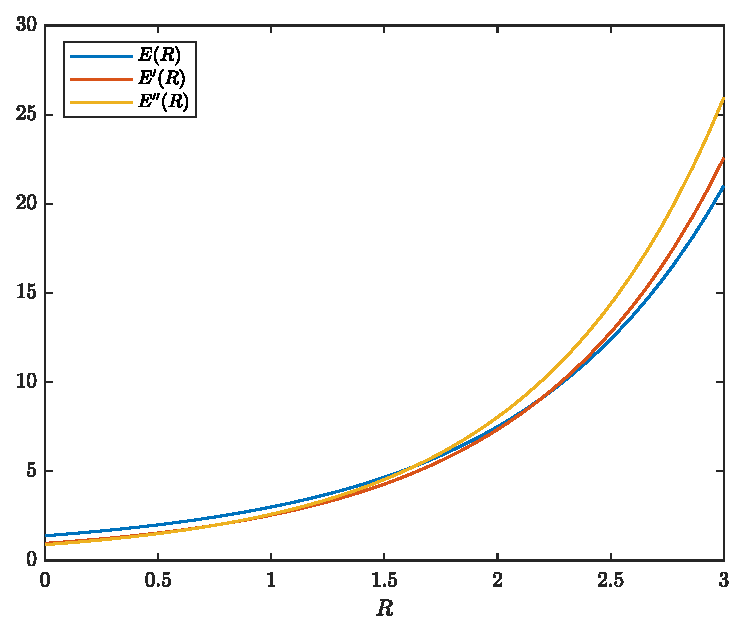
\includegraphics[width=0.7\linewidth]{img/energy_per_bit_1.eps}
	\caption{$E_b(R)$, $E'_b(R)$, $E''_b(R)$ for $R < \frac{1}{2} \log\Big(\frac{g_2^2}{g_1^2}\Big)$ }
	\label{fig:funcex2}
\end{figure}


Now we want to compute the minimum energy-per-bit as $R \rightarrow 0$. We notice that for low values of $R$ we find ourself in the case where only one of the two channels is opened. We conclude that the minimum energy-per-bit as $R \rightarrow 0$ is equal to \eqref{emin}.

\begin{equation}
	\lim_{R \rightarrow 0} E_b(R) =
		\lim_{R \rightarrow 0} \Big(\frac{2^{2R}-1}{g_2^2 R}\Big) = \lim_{R \rightarrow 0} \frac{ \frac{d(2^{2R}-1)}{dR}} {\frac{dg_2^2 R}{dR}}=\frac{2\ln{2}}{g_2^2}
		\label{emin}
\end{equation}

\numberwithin{equation}{section}
